% Compile with: pdflatex architecture.tex
% Requires: tikz, booktabs, lmodern, microtype (all standard in TeX Live / MiKTeX)
\documentclass[10pt,a4paper]{article}
\usepackage[top=1.15cm, bottom=1.15cm, left=1.4cm, right=1.4cm]{geometry}
\usepackage{tikz}
\usetikzlibrary{arrows.meta}
\usepackage{booktabs}
\usepackage{xcolor}
\usepackage[T1]{fontenc}
\usepackage{lmodern}
\usepackage{microtype}
\usepackage{tabularx}
\usepackage{array}

% ── Colour palette ──────────────────────────────────────────────────────────
\definecolor{cblue}  {HTML}{1565C0}   % Spring Boot / primary
\definecolor{clblue} {HTML}{1976D2}   % Angular
\definecolor{cteal}  {HTML}{00796B}   % Playwright
\definecolor{corange}{HTML}{BF360C}   % K6 / security accent
\definecolor{cpurple}{HTML}{6A1B9A}   % JWT + RBAC
\definecolor{cgray}  {HTML}{546E7A}   % data layer
\definecolor{cbg}    {HTML}{FAFAFA}   % box fill base

\setlength{\parindent}{0pt}
\pagestyle{empty}

\begin{document}

% ═══════════════════════════════════════════════════════════════════════════
%  HEADER
% ═══════════════════════════════════════════════════════════════════════════
\begin{center}
  {\large\bfseries\color{cblue}Release Management Tool (RMT) — Testing Architecture}\\[2pt]
  {\small
    SE3112 Advanced Software Engineering\quad\textbullet\quad
    Playwright\ (E2E / UI)\quad\textbullet\quad K6\ (Load / Performance)\quad\textbullet\quad
    Spring Boot 3 + Angular 17
  }
\end{center}
\noindent\rule{\linewidth}{0.8pt}
\vspace{3pt}

% ═══════════════════════════════════════════════════════════════════════════
%  TWO-COLUMN BODY
% ═══════════════════════════════════════════════════════════════════════════
\begin{minipage}[t]{0.55\textwidth}

{\small\bfseries\color{cblue}System Architecture \& Test Coverage}

\vspace{5pt}

% ── Architecture diagram ──────────────────────────────────────────────────
%
%  Node centres (x, y):
%    pw   (1.375,  0.0)   Playwright    – tbox 2.55 × 0.60
%    k6   (4.375,  0.0)   K6            – tbox 2.55 × 0.60
%    ng   (2.875, -1.4)   Angular       – wbox 5.50 × 0.60
%    api  (2.875, -2.8)   Spring Boot   – wbox 5.50 × 0.60
%    jwt  (1.375, -4.2)   JWT+RBAC      – sbox 2.55 × 0.60
%    sm   (4.375, -4.2)   State Machine – sbox 2.55 × 0.60
%    db   (1.375, -5.6)   MySQL 8       – sbox 2.55 × 0.60
%    fly  (4.375, -5.6)   Flyway        – sbox 2.55 × 0.60
%
%  Key derived anchors:
%    pw.south  = (1.375, -0.30)   ng.north  = (*,    -1.10)
%    ng.south  = (2.875, -1.70)   api.north = (2.875,-2.50)
%    api.south = (*,     -3.10)   api.east  = (5.625,-2.80)
%    jwt.north = (1.375, -3.90)   sm.north  = (4.375,-3.90)
%    jwt.south = (1.375, -4.50)   sm.south  = (4.375,-4.50)
%    db.north  = (1.375, -5.30)   fly.north = (4.375,-5.30)
%
%  K6 bypass path (right → down → left, outside Angular):
%    k6.south(4.375,-0.30) → (5.95,-0.30) → (5.95,-2.80) → api.east(5.625,-2.80)
%
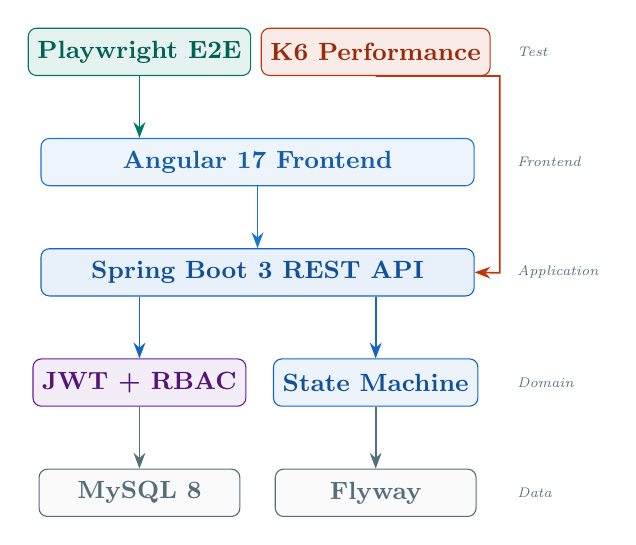
\begin{tikzpicture}[
  arr/.style  = {-Stealth, semithick},
  tbox/.style = {rectangle, rounded corners=3pt,
                 minimum width=2.55cm, minimum height=0.60cm,
                 text centered, font=\small\bfseries},
  wbox/.style = {tbox, minimum width=5.50cm},
  sbox/.style = {tbox, minimum width=2.55cm}
]

%% ── Nodes ─────────────────────────────────────────────────────────────────
\node[tbox, draw=cteal,   fill=cteal!10,   text=cteal!80!black]  (pw)  at (1.375,  0.0) {Playwright E2E};
\node[tbox, draw=corange, fill=corange!10, text=corange!80!black](k6)  at (4.375,  0.0) {K6 Performance};
\node[wbox, draw=clblue,  fill=clblue!8,   text=clblue!80!black] (ng)  at (2.875, -1.4) {Angular 17 Frontend};
\node[wbox, draw=cblue,   fill=cblue!10,   text=cblue!80!black]  (api) at (2.875, -2.8) {Spring Boot 3 REST API};
\node[sbox, draw=cpurple, fill=cpurple!8,  text=cpurple!80!black](jwt) at (1.375, -4.2) {JWT + RBAC};
\node[sbox, draw=cblue,   fill=cblue!8,    text=cblue!80!black]  (sm)  at (4.375, -4.2) {State Machine};
\node[sbox, draw=cgray,   fill=cbg,        text=cgray]           (db)  at (1.375, -5.6) {MySQL 8};
\node[sbox, draw=cgray,   fill=cbg,        text=cgray]           (fly) at (4.375, -5.6) {Flyway};

%% ── Arrows ────────────────────────────────────────────────────────────────
% Playwright → Angular (vertical)
\draw[arr, color=cteal]
  (pw.south) -- (pw.south |- ng.north);

% K6 → Spring Boot  (bypass Angular: right → down → left)
\draw[arr, color=corange]
  (k6.south) -- ++(1.575, 0) -- ++(0, -2.50) -- (api.east);

% Angular → Spring Boot (vertical)
\draw[arr, color=clblue]
  (ng.south) -- (api.north);

% Spring Boot → JWT + RBAC  (spring south-border at jwt's x → jwt top)
\draw[arr, color=cblue]
  (jwt.north |- api.south) -- (jwt.north);

% Spring Boot → State Machine  (spring south-border at sm's x → sm top)
\draw[arr, color=cblue]
  (sm.north |- api.south) -- (sm.north);

% JWT → MySQL
\draw[arr, color=cgray]  (jwt.south) -- (db.north);

% State Machine → Flyway
\draw[arr, color=cgray]  (sm.south)  -- (fly.north);

%% ── Layer labels (right margin) ───────────────────────────────────────────
\node[font=\tiny\itshape, text=cgray, anchor=west] at (6.05,  0.0) {Test};
\node[font=\tiny\itshape, text=cgray, anchor=west] at (6.05, -1.4) {Frontend};
\node[font=\tiny\itshape, text=cgray, anchor=west] at (6.05, -2.8) {Application};
\node[font=\tiny\itshape, text=cgray, anchor=west] at (6.05, -4.2) {Domain};
\node[font=\tiny\itshape, text=cgray, anchor=west] at (6.05, -5.6) {Data};

\end{tikzpicture}

\vspace{6pt}

{\small\bfseries\color{cblue}Release State Machine}\enspace
{\footnotesize\color{cgray}(ADMIN-only transitions)}

\vspace{4pt}


\begin{tikzpicture}[
  st/.style = {rectangle, rounded corners=3pt,
               minimum width=1.38cm, minimum height=0.50cm,
               text centered, font=\footnotesize\bfseries,
               draw=cblue, fill=cblue!10, text=cblue},
  arr/.style = {-Stealth, semithick, color=cblue}
]
\node[st] (d) at (0.00, 0) {DRAFT};
\node[st] (t) at (1.90, 0) {TESTING};
\node[st] (a) at (3.80, 0) {APPROVED};
\node[st] (r) at (5.70, 0) {RELEASED};
\draw[arr] (d) -- (t);
\draw[arr] (t) -- (a);
\draw[arr] (a) -- (r);
\end{tikzpicture}

\end{minipage}%
\hfill
% ── RIGHT COLUMN ────────────────────────────────────────────────────────────
\begin{minipage}[t]{0.42\textwidth}

{\small\bfseries\color{cblue}Tech Stack}

\vspace{3pt}

{\small
\begin{tabular}{@{}p{1.55cm}p{4.15cm}@{}}
Backend  & Java 17, Spring Boot 3.2, Spring Security (JWT + RBAC), Spring Data JPA, Flyway, MySQL 8 \\[3pt]
Frontend & Angular 17, RxJS, Angular Material, Chart.js \\[3pt]
Test DBs & H2 in-memory (unit)\,+\,MySQL (E2E) \\[3pt]
Features & State machine, AOP audit log, CSV export (\texttt{/api/releases/export.csv}) \\
\end{tabular}
}

\vspace{7pt}

{\small\bfseries\color{cblue}Tool Justification}

\vspace{3pt}

{\small
\begin{tabular}{@{}p{1.45cm}p{4.25cm}@{}}
\toprule
Tool & Rationale \\
\midrule
Playwright
  & Native auto-wait matches Angular's async lifecycle;
    Page Object Model separates selectors from logic;
    trace + video debugging; no WebDriver overhead \\[5pt]
K6
  & JavaScript-scriptable VU model; \texttt{SharedArray}
    for memory-efficient data-driven payloads;
    env-var parametrisation for CI/CD integration \\
\bottomrule
\end{tabular}
}

\vspace{7pt}

{\small\bfseries\color{cblue}Team Contributions}

\vspace{3pt}

{\footnotesize
\begin{tabular}{@{}p{0.28cm}p{1.20cm}p{4.18cm}@{}}
\toprule
& Tool & Feature Owned \\
\midrule
S1
  & Playwright
  & Page Object Model + E2E Release Lifecycle:
    state transitions DRAFT\,{\footnotesize$\to$}\,RELEASED,
    CSV export, audit log API verification \\[4pt]
S2
  & Playwright
  & RBAC Enforcement + Negative \& Edge Cases:
    viewer 403 checks, oversized-input rejection,
    unauthenticated route redirect \\[4pt]
S3
  & K6
  & Spike \& Stress Configurations:
    gradual ramp to 150 VUs (stress),
    instant burst to 250 VUs (spike),
    saturation and recovery analysis \\[4pt]
S4
  & K6
  & Data-Driven Payload Testing:
    \texttt{SharedArray} with 10 release templates,
    POST\,+\,GET read-back integrity assertion,
    \texttt{checks rate\,>\,95\%} threshold \\
\bottomrule
\end{tabular}
}

\vspace{7pt}

{\small\bfseries\color{cblue}K6 Performance Results}

\vspace{3pt}

{\small
\begin{tabular}{@{}lrrrr@{}}
\toprule
Profile & VUs & Req/s & p95 (ms) & Fail \\
\midrule
Load   &  75 & 3\,396 &  54.69 & 0.00\% \\
Stress & 150 & 3\,081 &  73.23 & 0.00\% \\
Spike  & 250 & 2\,902 & 158.35 & 0.00\% \\
Write  &  60 & 2\,266 &  28.55 & 0.00\% \\
\midrule
\multicolumn{5}{@{}l@{}}{\footnotesize\color{cgray}All checks: 100\%\quad Playwright E2E: 5/5 passed} \\
\bottomrule
\end{tabular}
}

\end{minipage}

% ═══════════════════════════════════════════════════════════════════════════
%  FOOTER
% ═══════════════════════════════════════════════════════════════════════════
\vspace{4pt}
\noindent\rule{\linewidth}{0.5pt}
{\footnotesize\color{cgray}
  \textbf{No Selenium\,·\,No Postman}\enskip
  Playwright 1.53 drives a real Chromium browser against the live Angular\,+\,Spring stack
  (auto-started via \texttt{playwright.config.ts}).\enskip
  K6 sends concurrent HTTP requests directly to the REST API using a goroutine-per-VU execution model.
}

\end{document}
